\section{Results}
\subsection{Motion captured chewing trajectories}
\label{sec:traj_result}

Figure~\ref{fig:trajectory_plot} shows a trajectory obtained using the method described in Section~\ref{sec:motion-capture}. The vertical displacement clearly reveals cyclic jaw movements, 
identifiable by recurring peaks that correspond to the opening and closing 
phases of the chewing cycle. The horizontal components (x and y) show a pattern consistent with reported human data \cite{chewing_traj}.

The orientation data on the other hand is less reliable as no clear pattern can be seen throughout the trajectory. Several factors described in Section~\ref{sec:motion_capture_limitations} 
may contribute to this inaccuracy. 

Nonetheless, the trajectory remains sufficiently accurate to evaluate the robot's position control performance and serves as a useful initial 
benchmark.

% \begin{figure}[H]
% \centering
% \begin{minipage}{.45\textwidth}
%   \centering
%   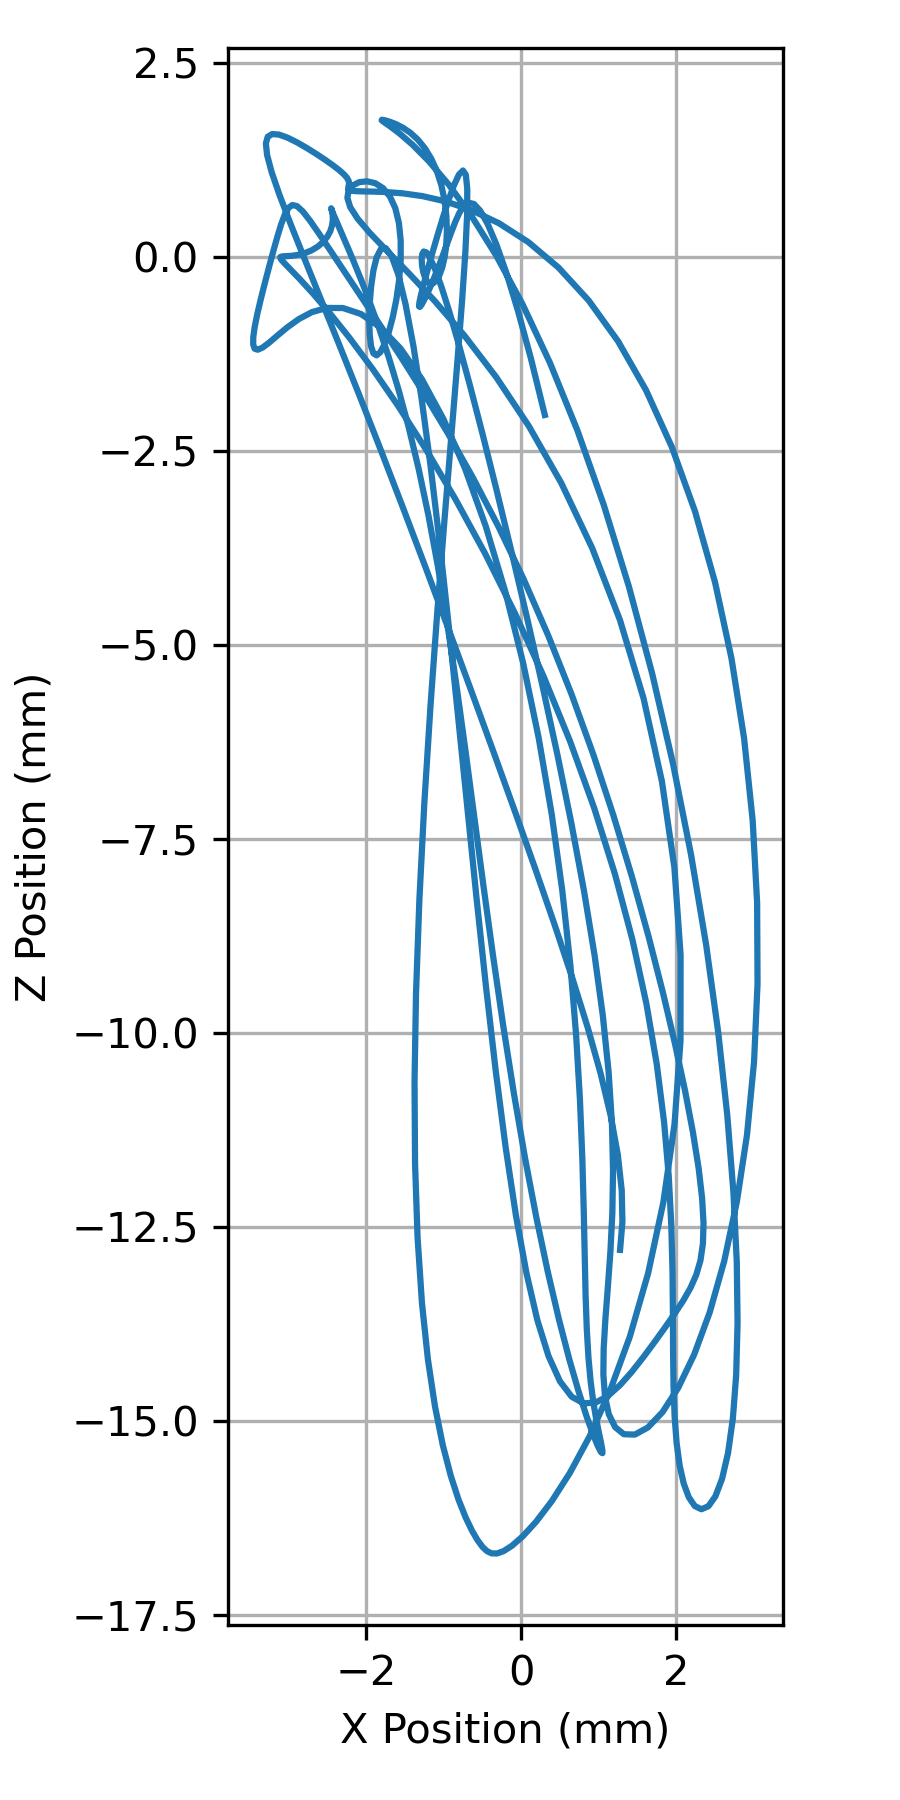
\includegraphics[height=6cm]{figures/x_vs_z_position.png}
%   \subcaption{}
%   \label{fig:x-z}
% \end{minipage}
% \begin{minipage}{.45\textwidth}
%   \centering
%   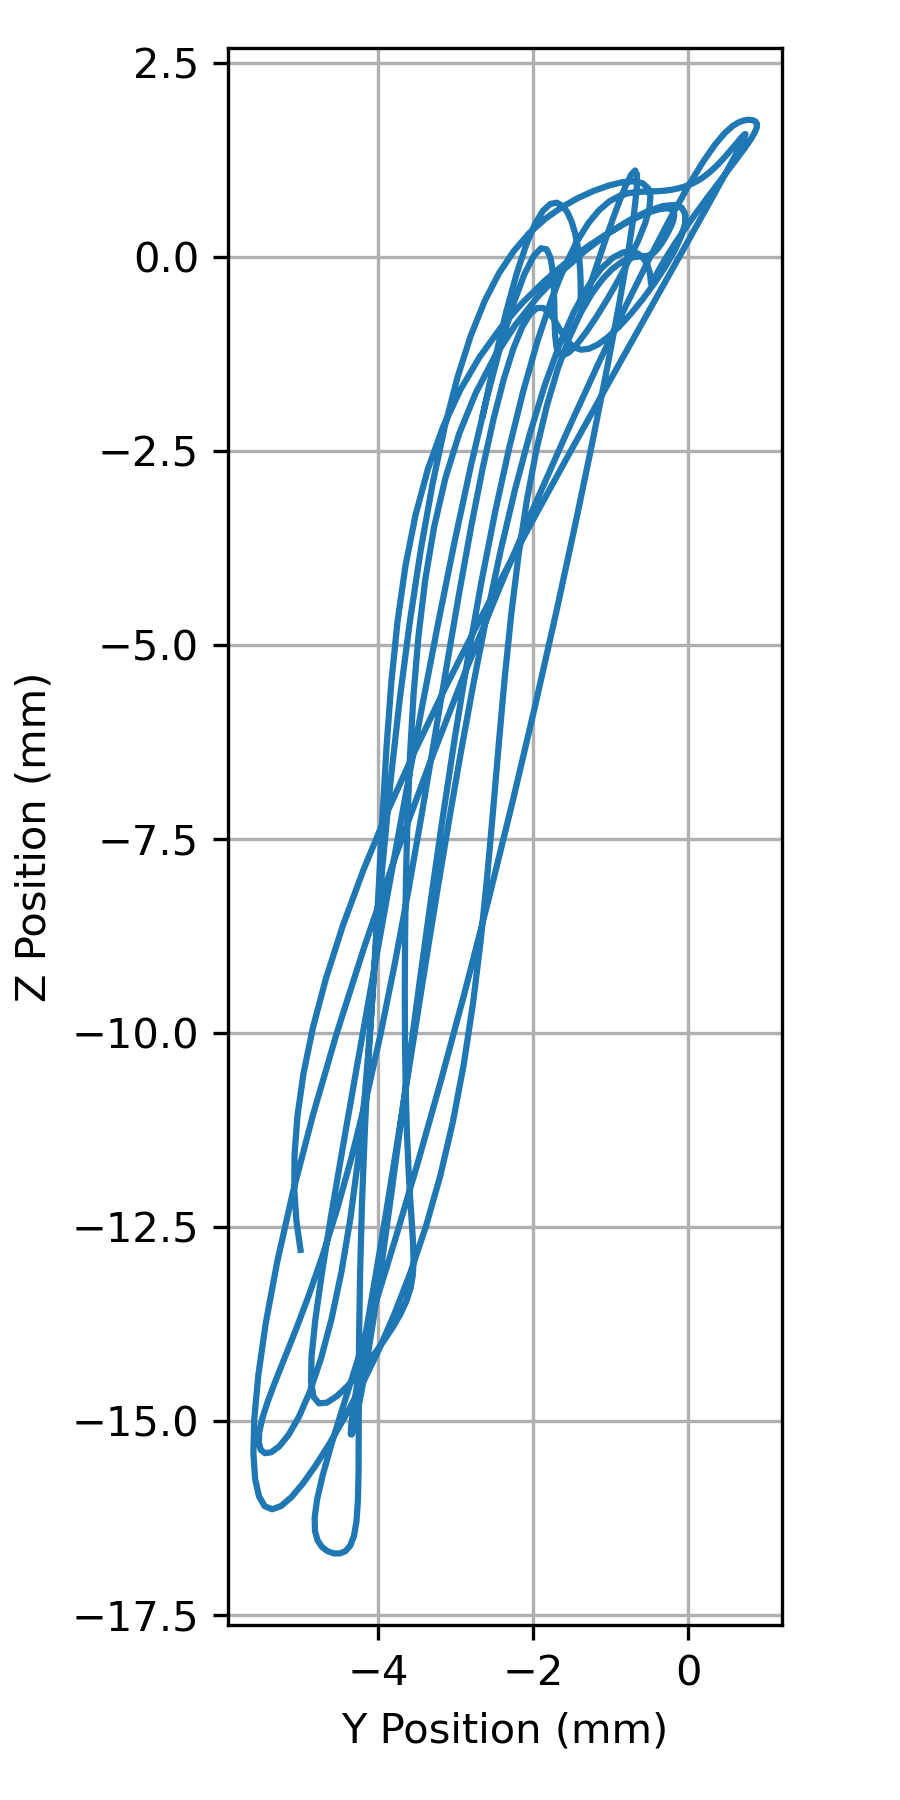
\includegraphics[height=6cm]{figures/y_vs_z_position.png}
%   \subcaption{}
%   \label{fig:y-z}
% \end{minipage}
% \caption{Position of the jaw in the x-z plane (a) and y-z plane (b).}
% \label{fig:xy-z}
% \end{figure}

\begin{figure}[H]
    \centering
    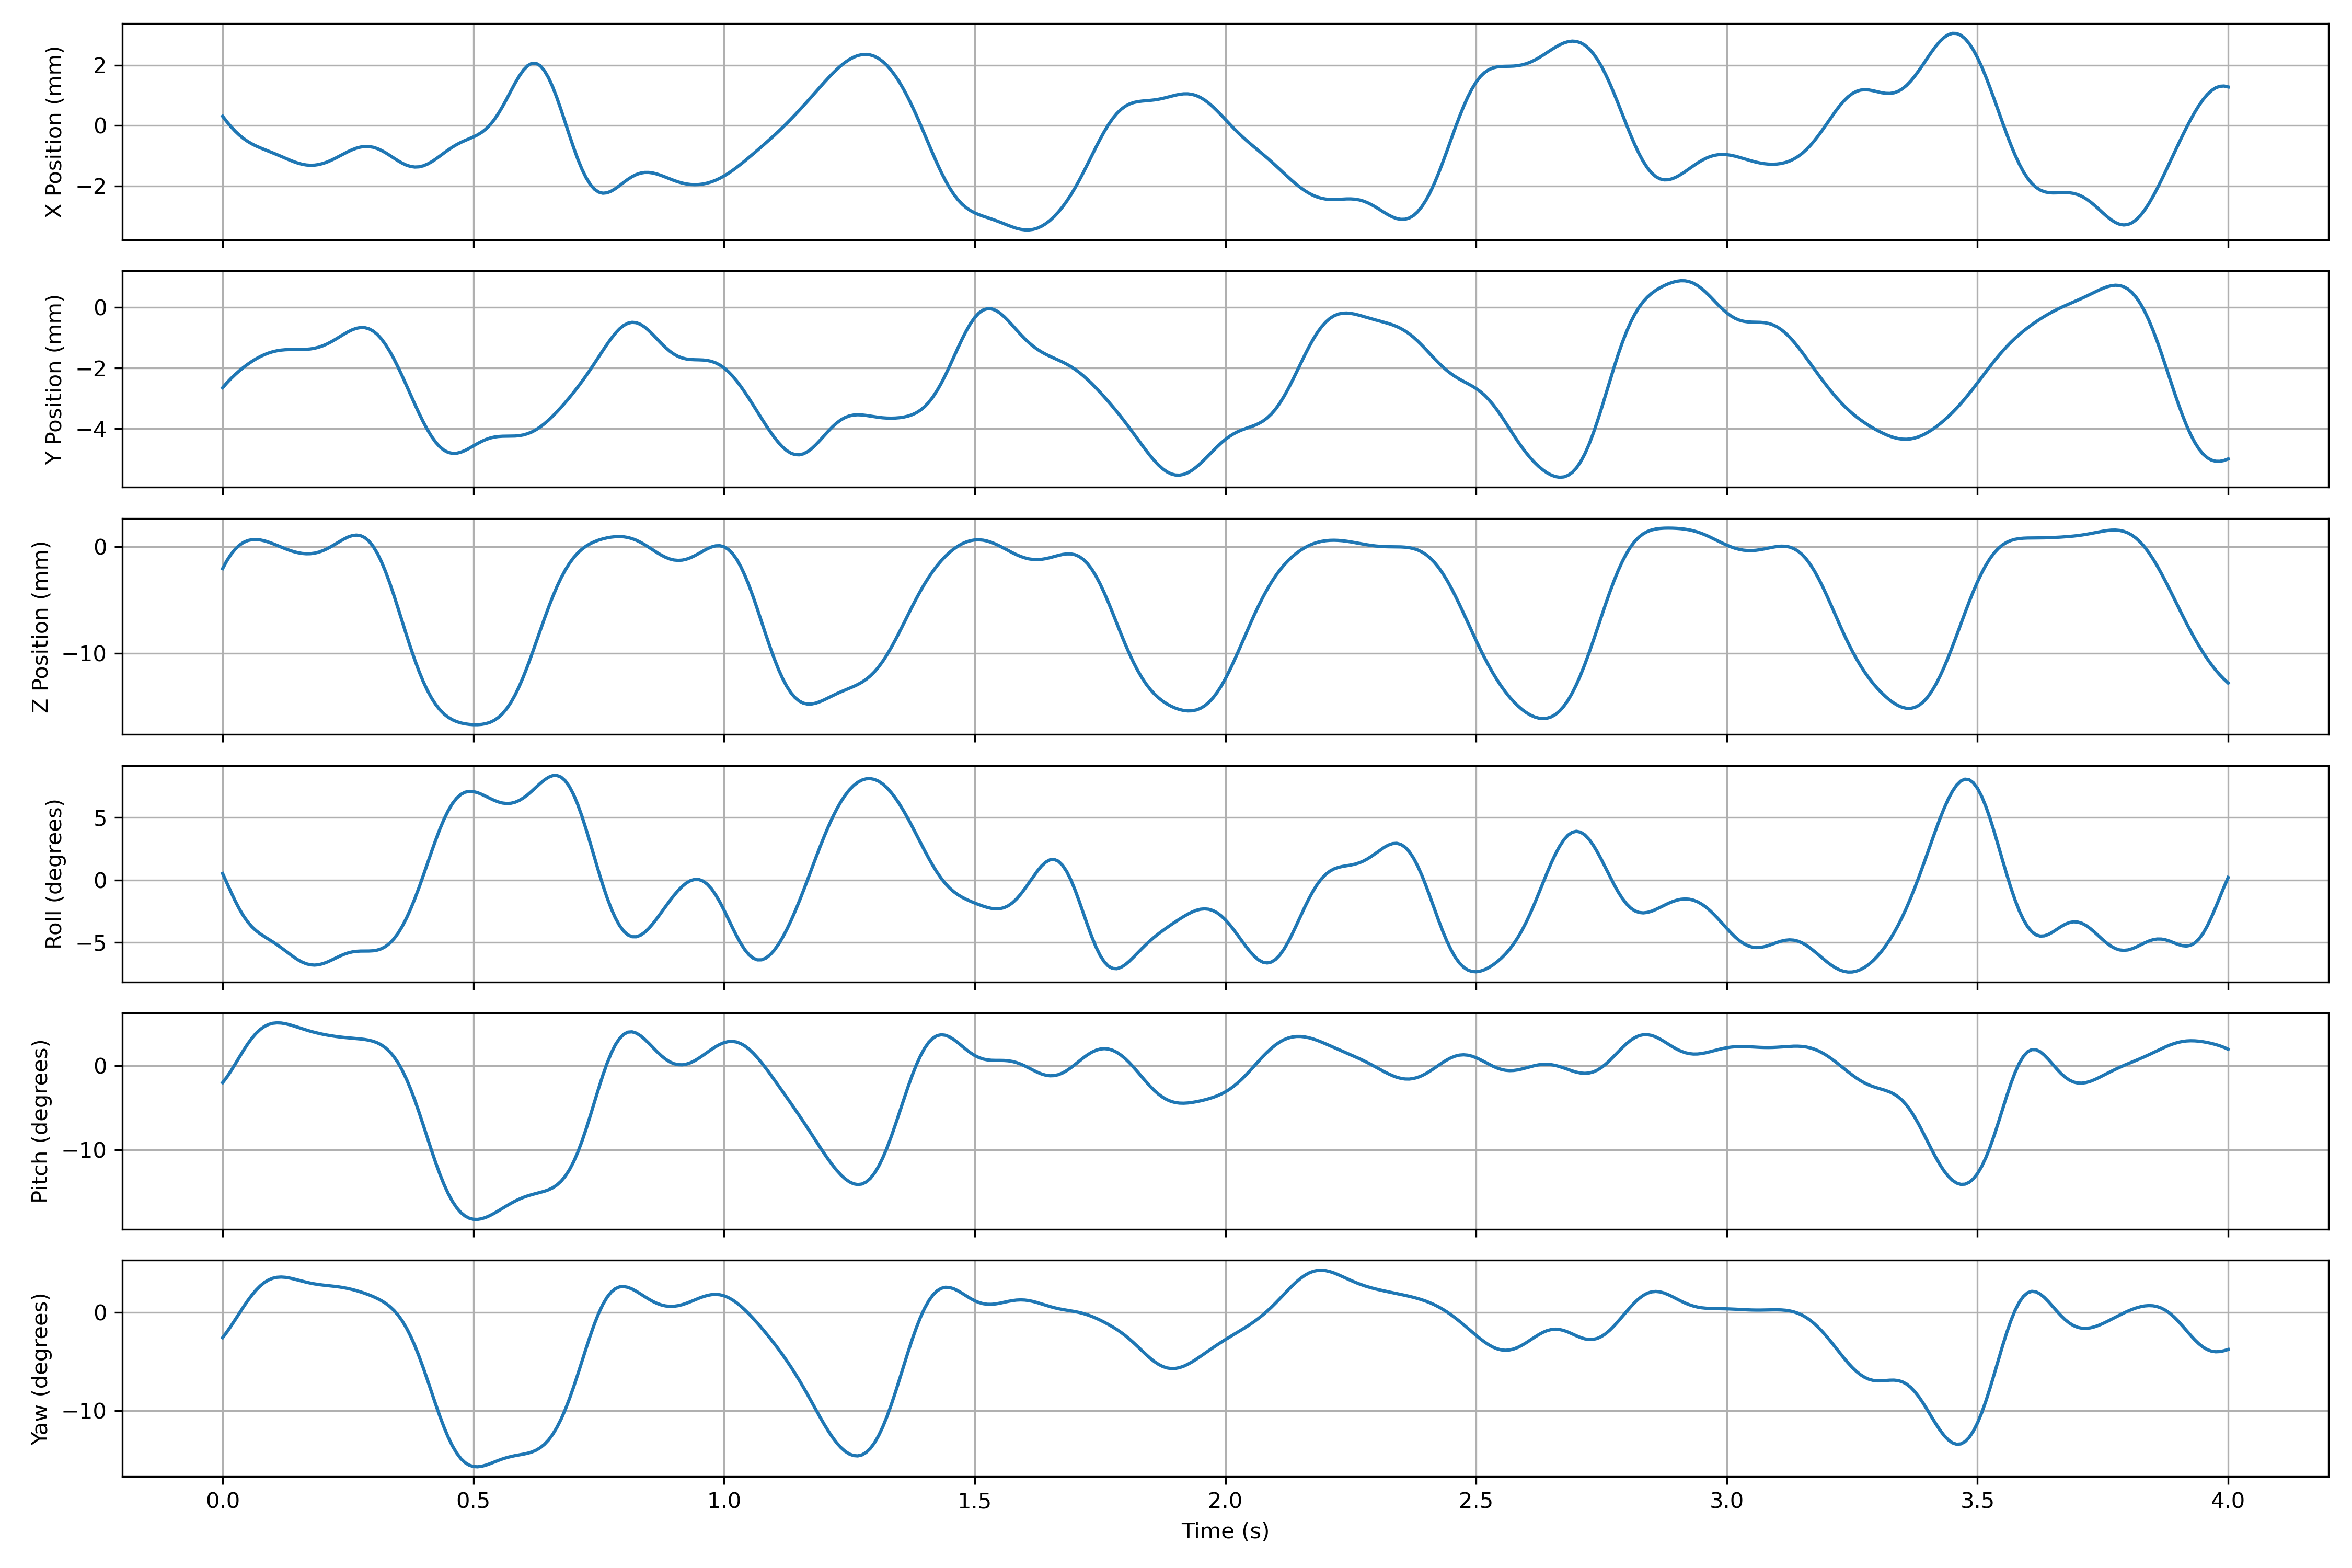
\includegraphics[width=\textwidth]{figures/trajectory_plot.png}
    \caption{Random side chewing gum mastication trajectory.}
    \label{fig:trajectory_plot}
\end{figure}

\subsection{Position control}

To evaluate the performance of the position control system, we investigated the robot's ability to track a predefined trajectory at varying speeds. 
In this context, “speed” refers to the time interval between consecutive trajectory points. While the motion capture data was recorded at 120 Hz 
(approximately every 8.3 ms), the playback was tested at longer intervals: 40 ms (25 Hz), 50 ms (20 Hz), 60 ms (16.67 Hz), 70 ms (14.29 Hz), 80 ms 
(12.5 Hz), 90 ms (11.11 Hz), and 100 ms (10 Hz).

For this test, a 10-second segment of chewing motion was used. Figure~\ref{fig:actuator_delays_2} illustrates the tracking performance of actuator 2 
at the various speeds. To quantify timing discrepancies, we conducted a cross-correlation analysis between the target and actual actuator lengths, 
providing both time delays (Figure~\ref{fig:actuator_delays_2}) and cross-correlation coefficients (Figure~\ref{fig:actuator_rhos_2}).

The results show that at a sampling interval of 100 ms (10 Hz), the robot tracks the trajectory well, with an average delay of ~0.7 s and 
cross-correlation coefficients exceeding 0.975. However, performance degrades significantly at higher speeds (i.e., shorter intervals), 
as reflected in both increased delays and a drop in correlation values—especially below 80 ms, where the tracking error becomes pronounced 
and key trajectory peaks are missed.

\begin{figure}[H]
    \centering
    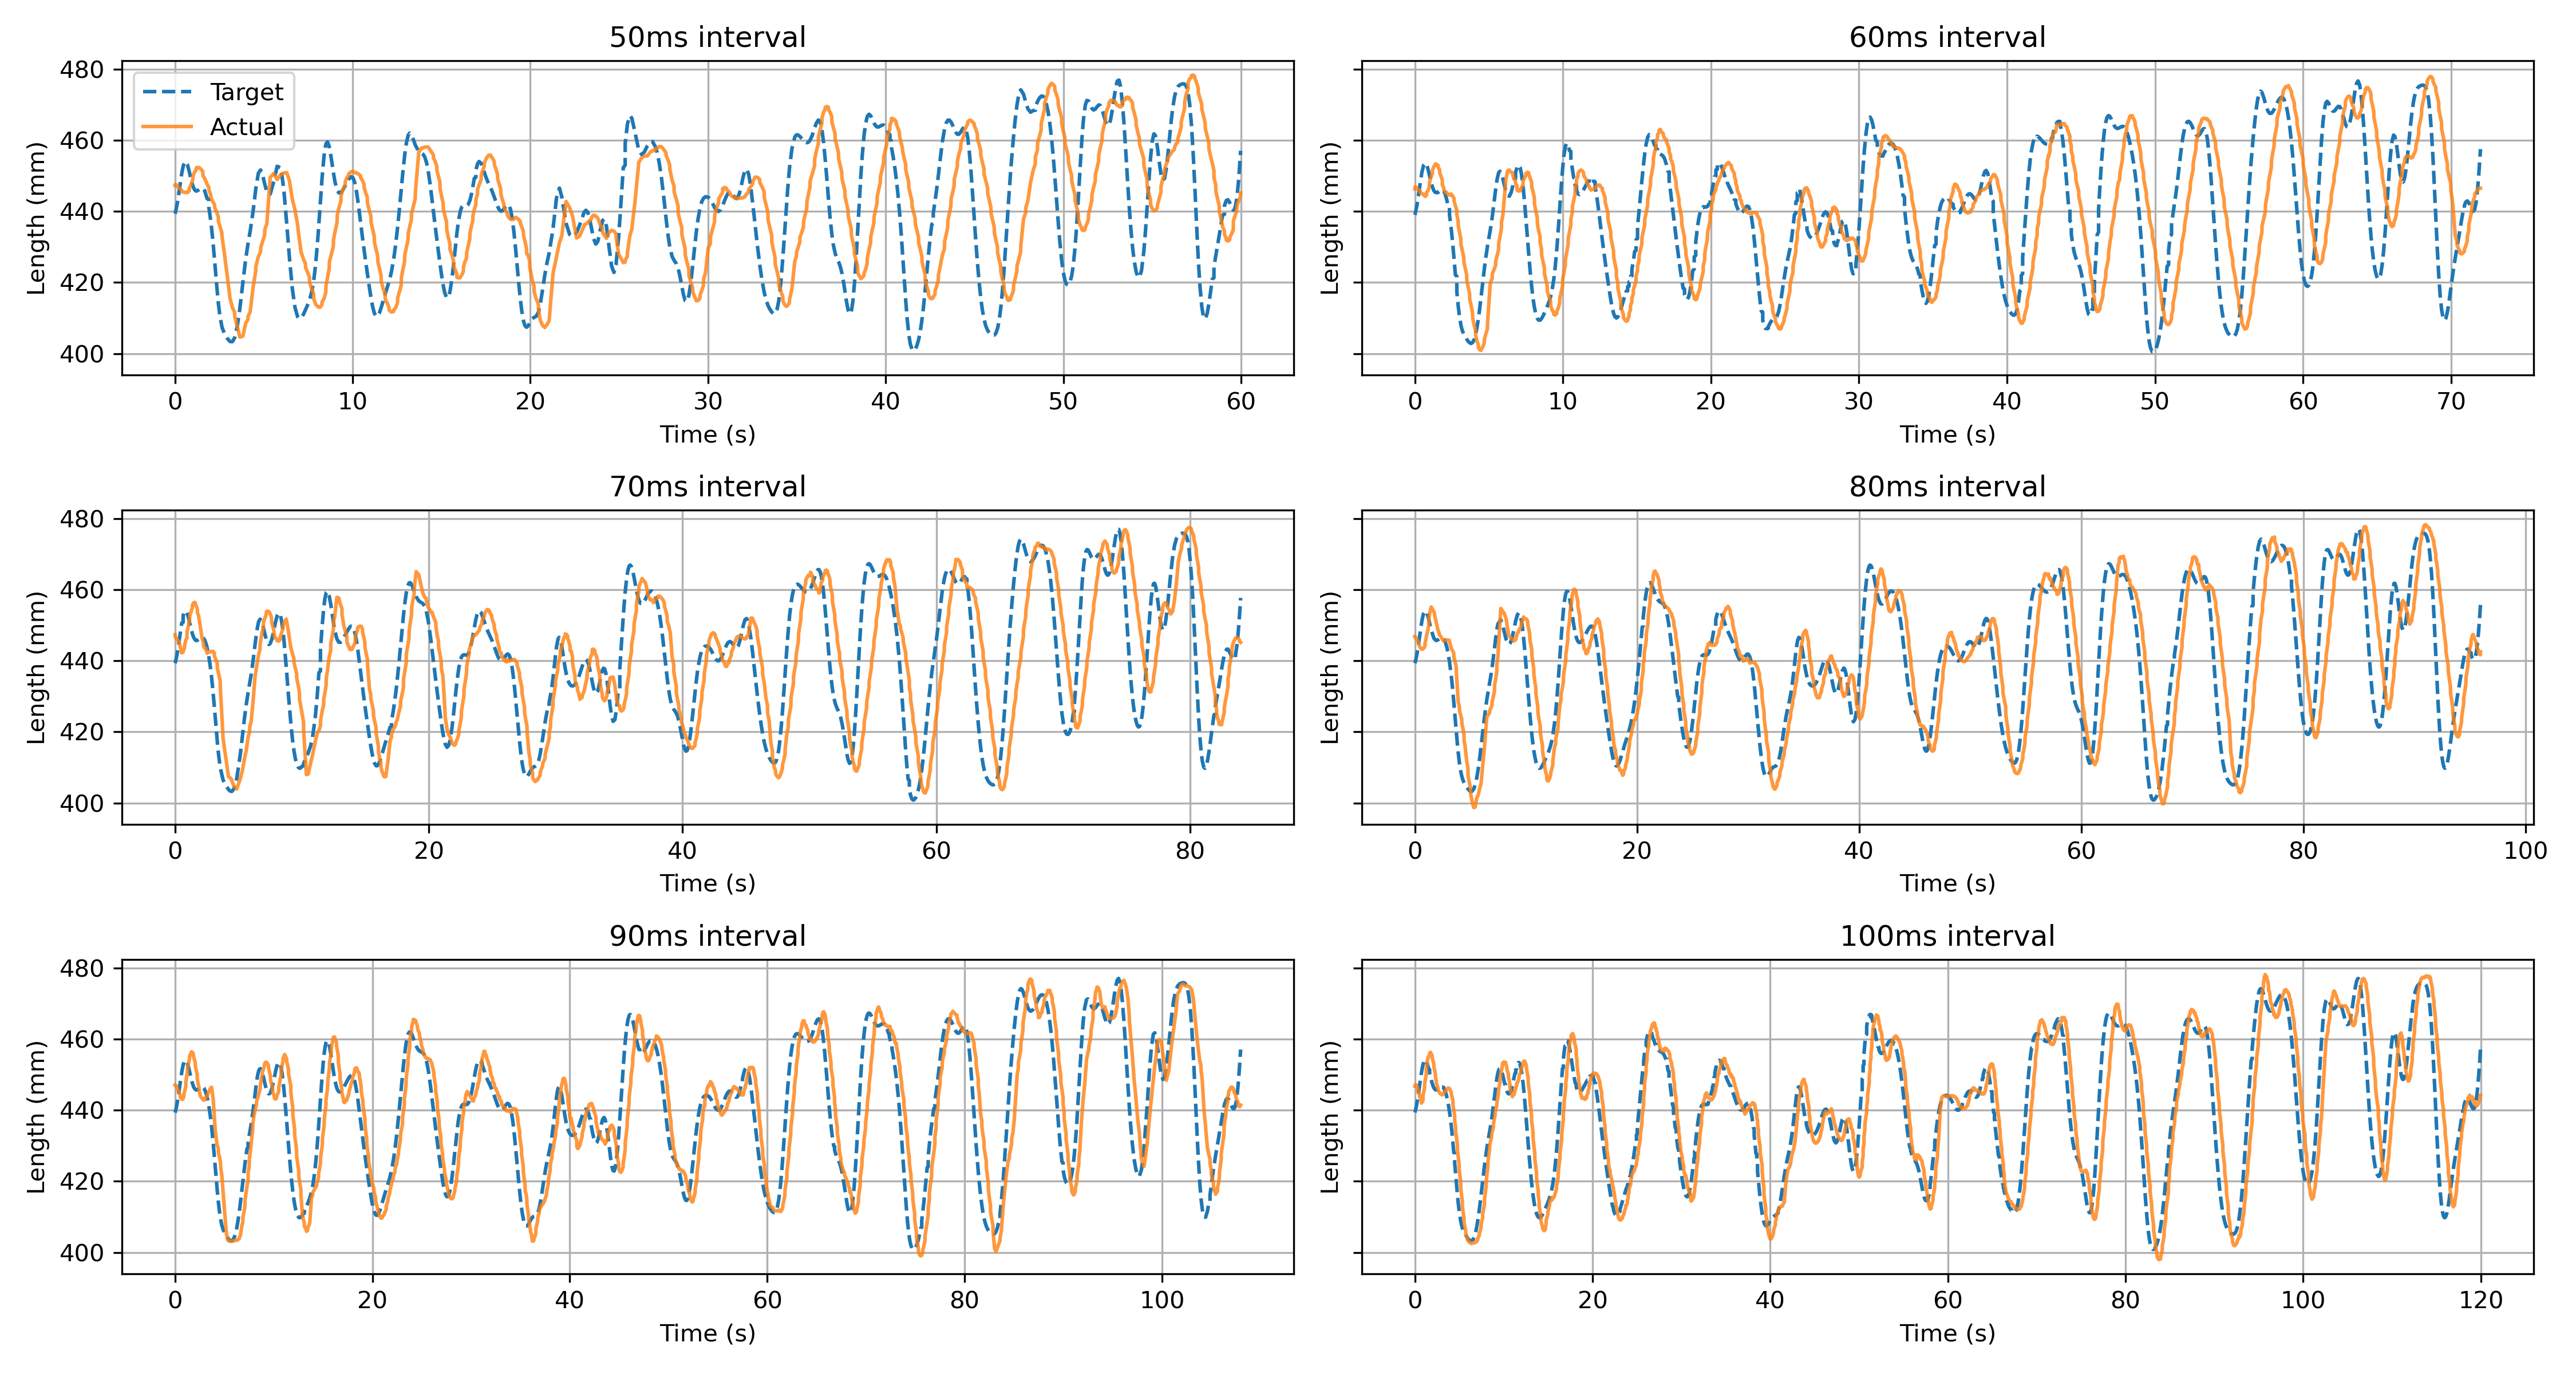
\includegraphics[width=\textwidth]{figures/actuator_2_trajectories.png}
    \caption{Performance of position control of actuator 2 across different time intervals between trajectory points.}
    \label{fig:position_control}
\end{figure}

\begin{figure}[H]
    \centering
    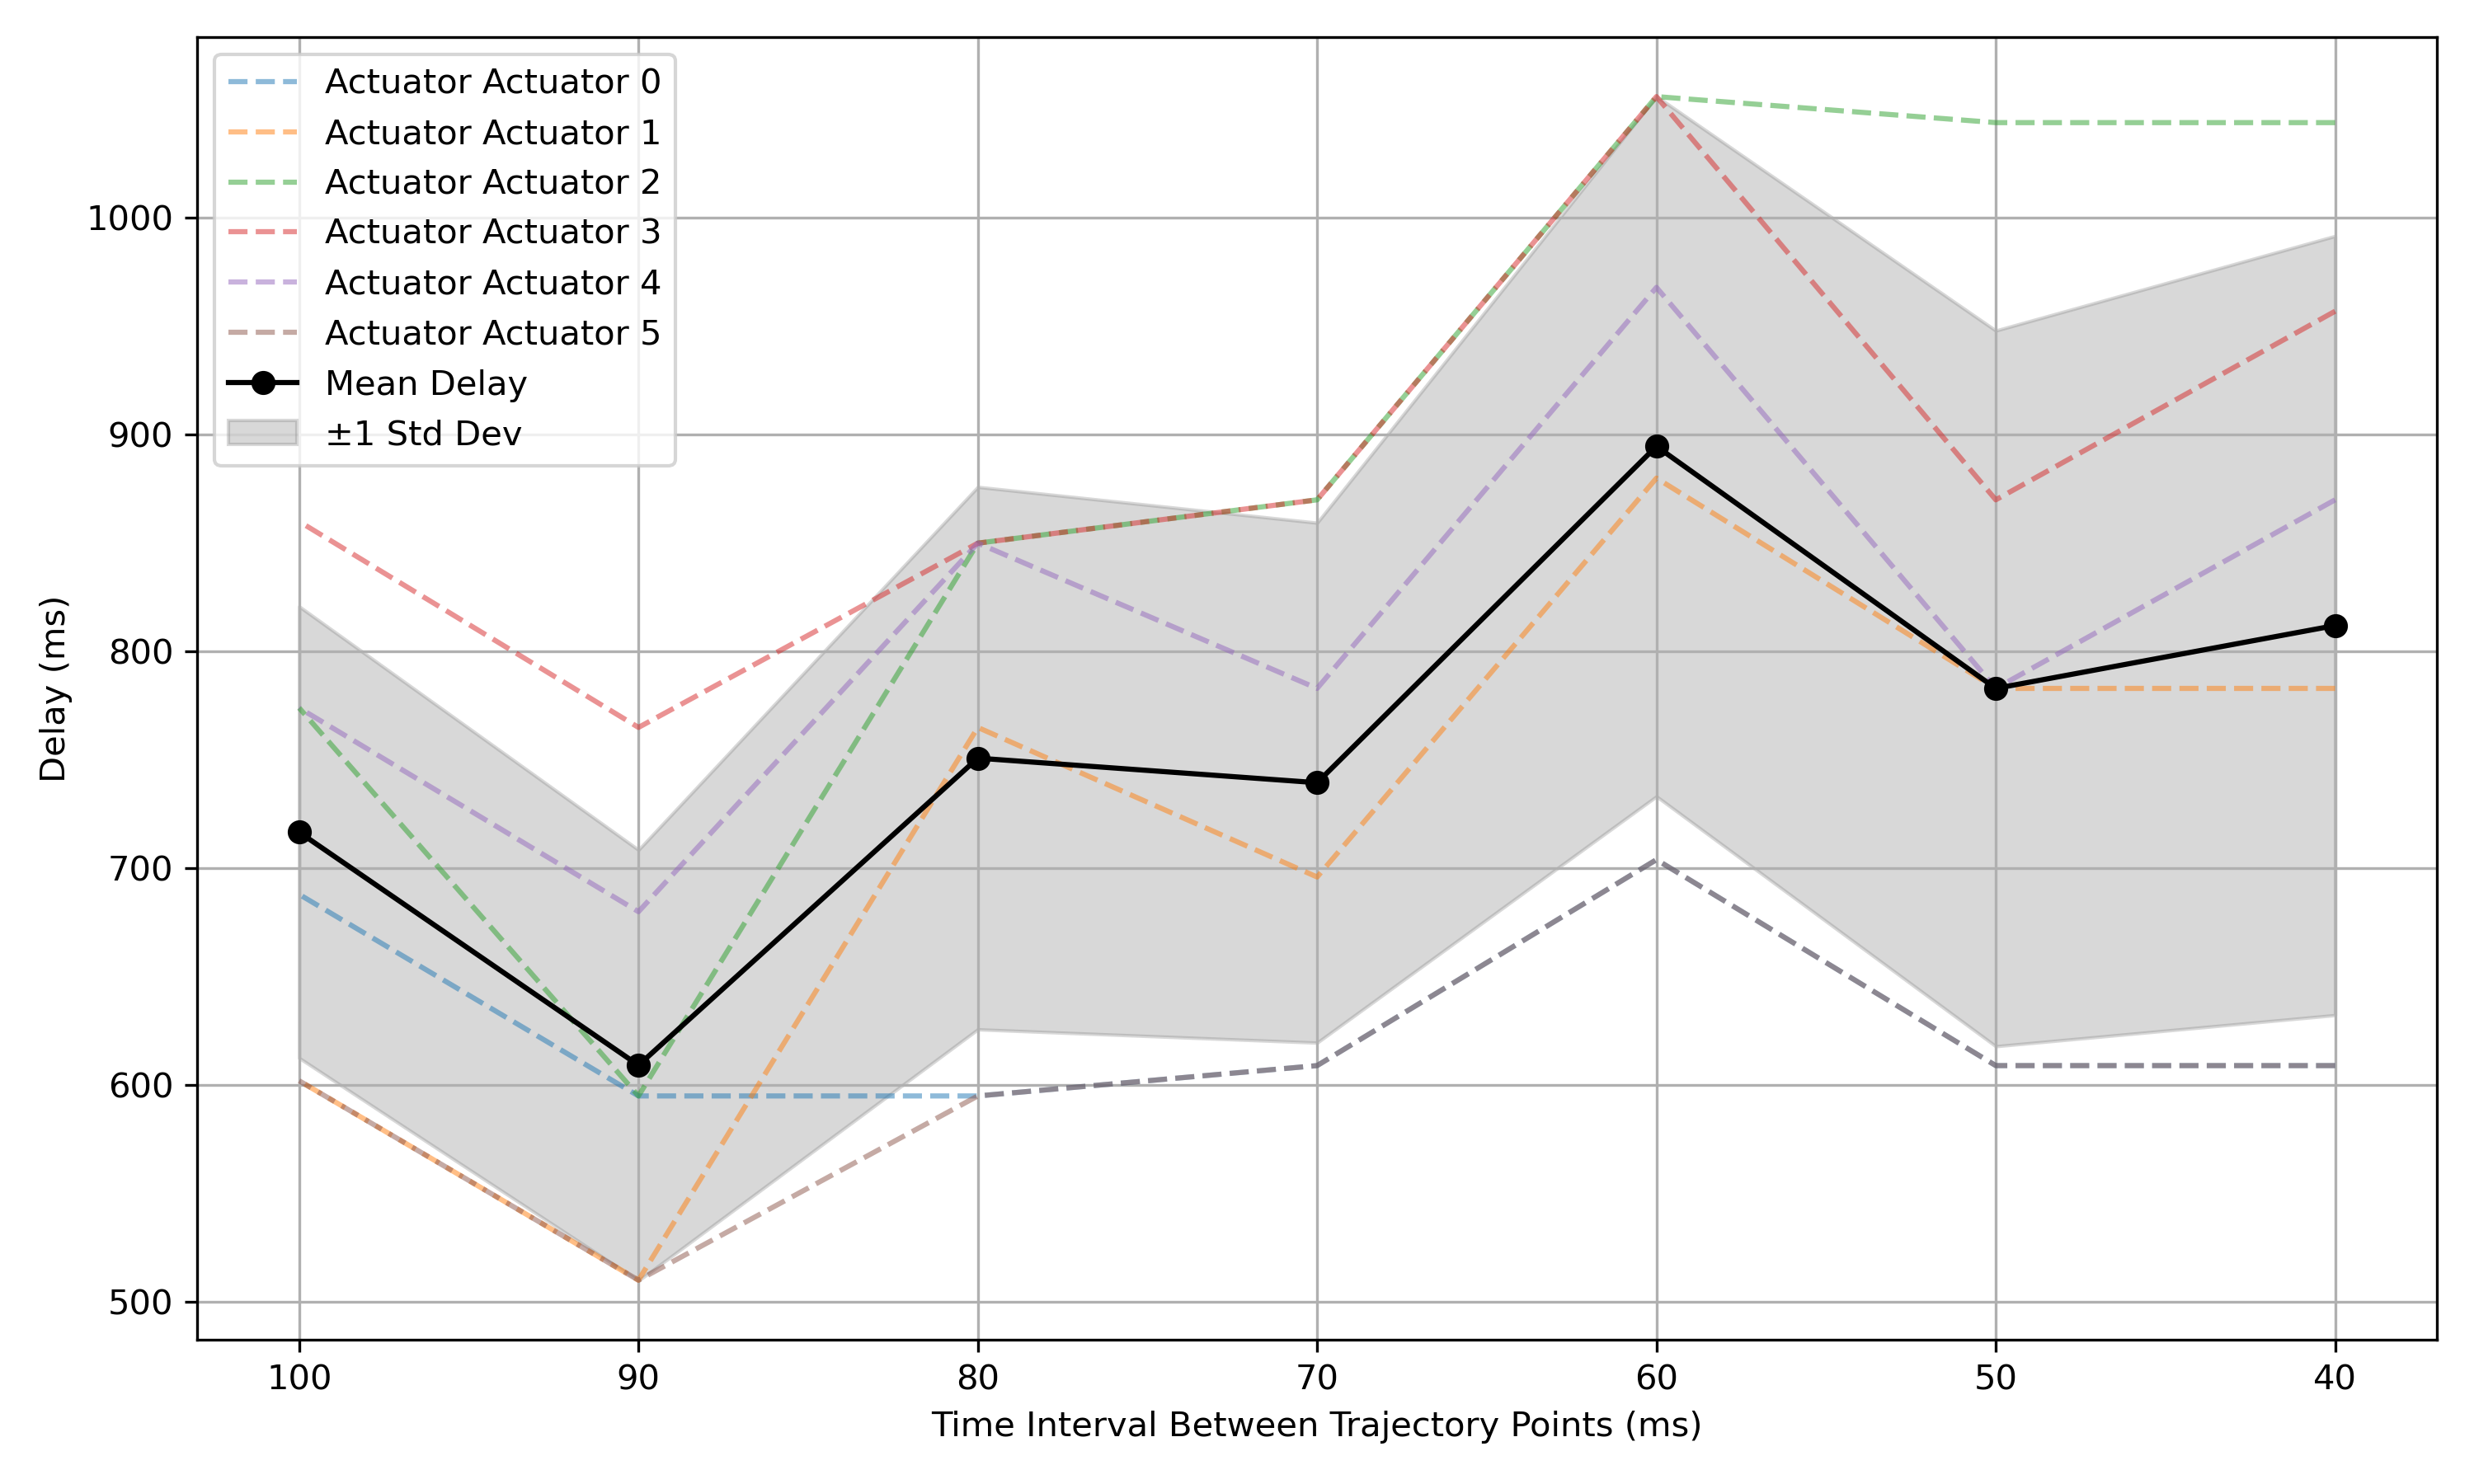
\includegraphics[width=0.6\textwidth]{figures/actuator_delays.png}
    \caption{Delays between target and actual actuator length across different time intervals.}
    \label{fig:actuator_delays_2}
\end{figure}

\begin{figure}[H]
    \centering
    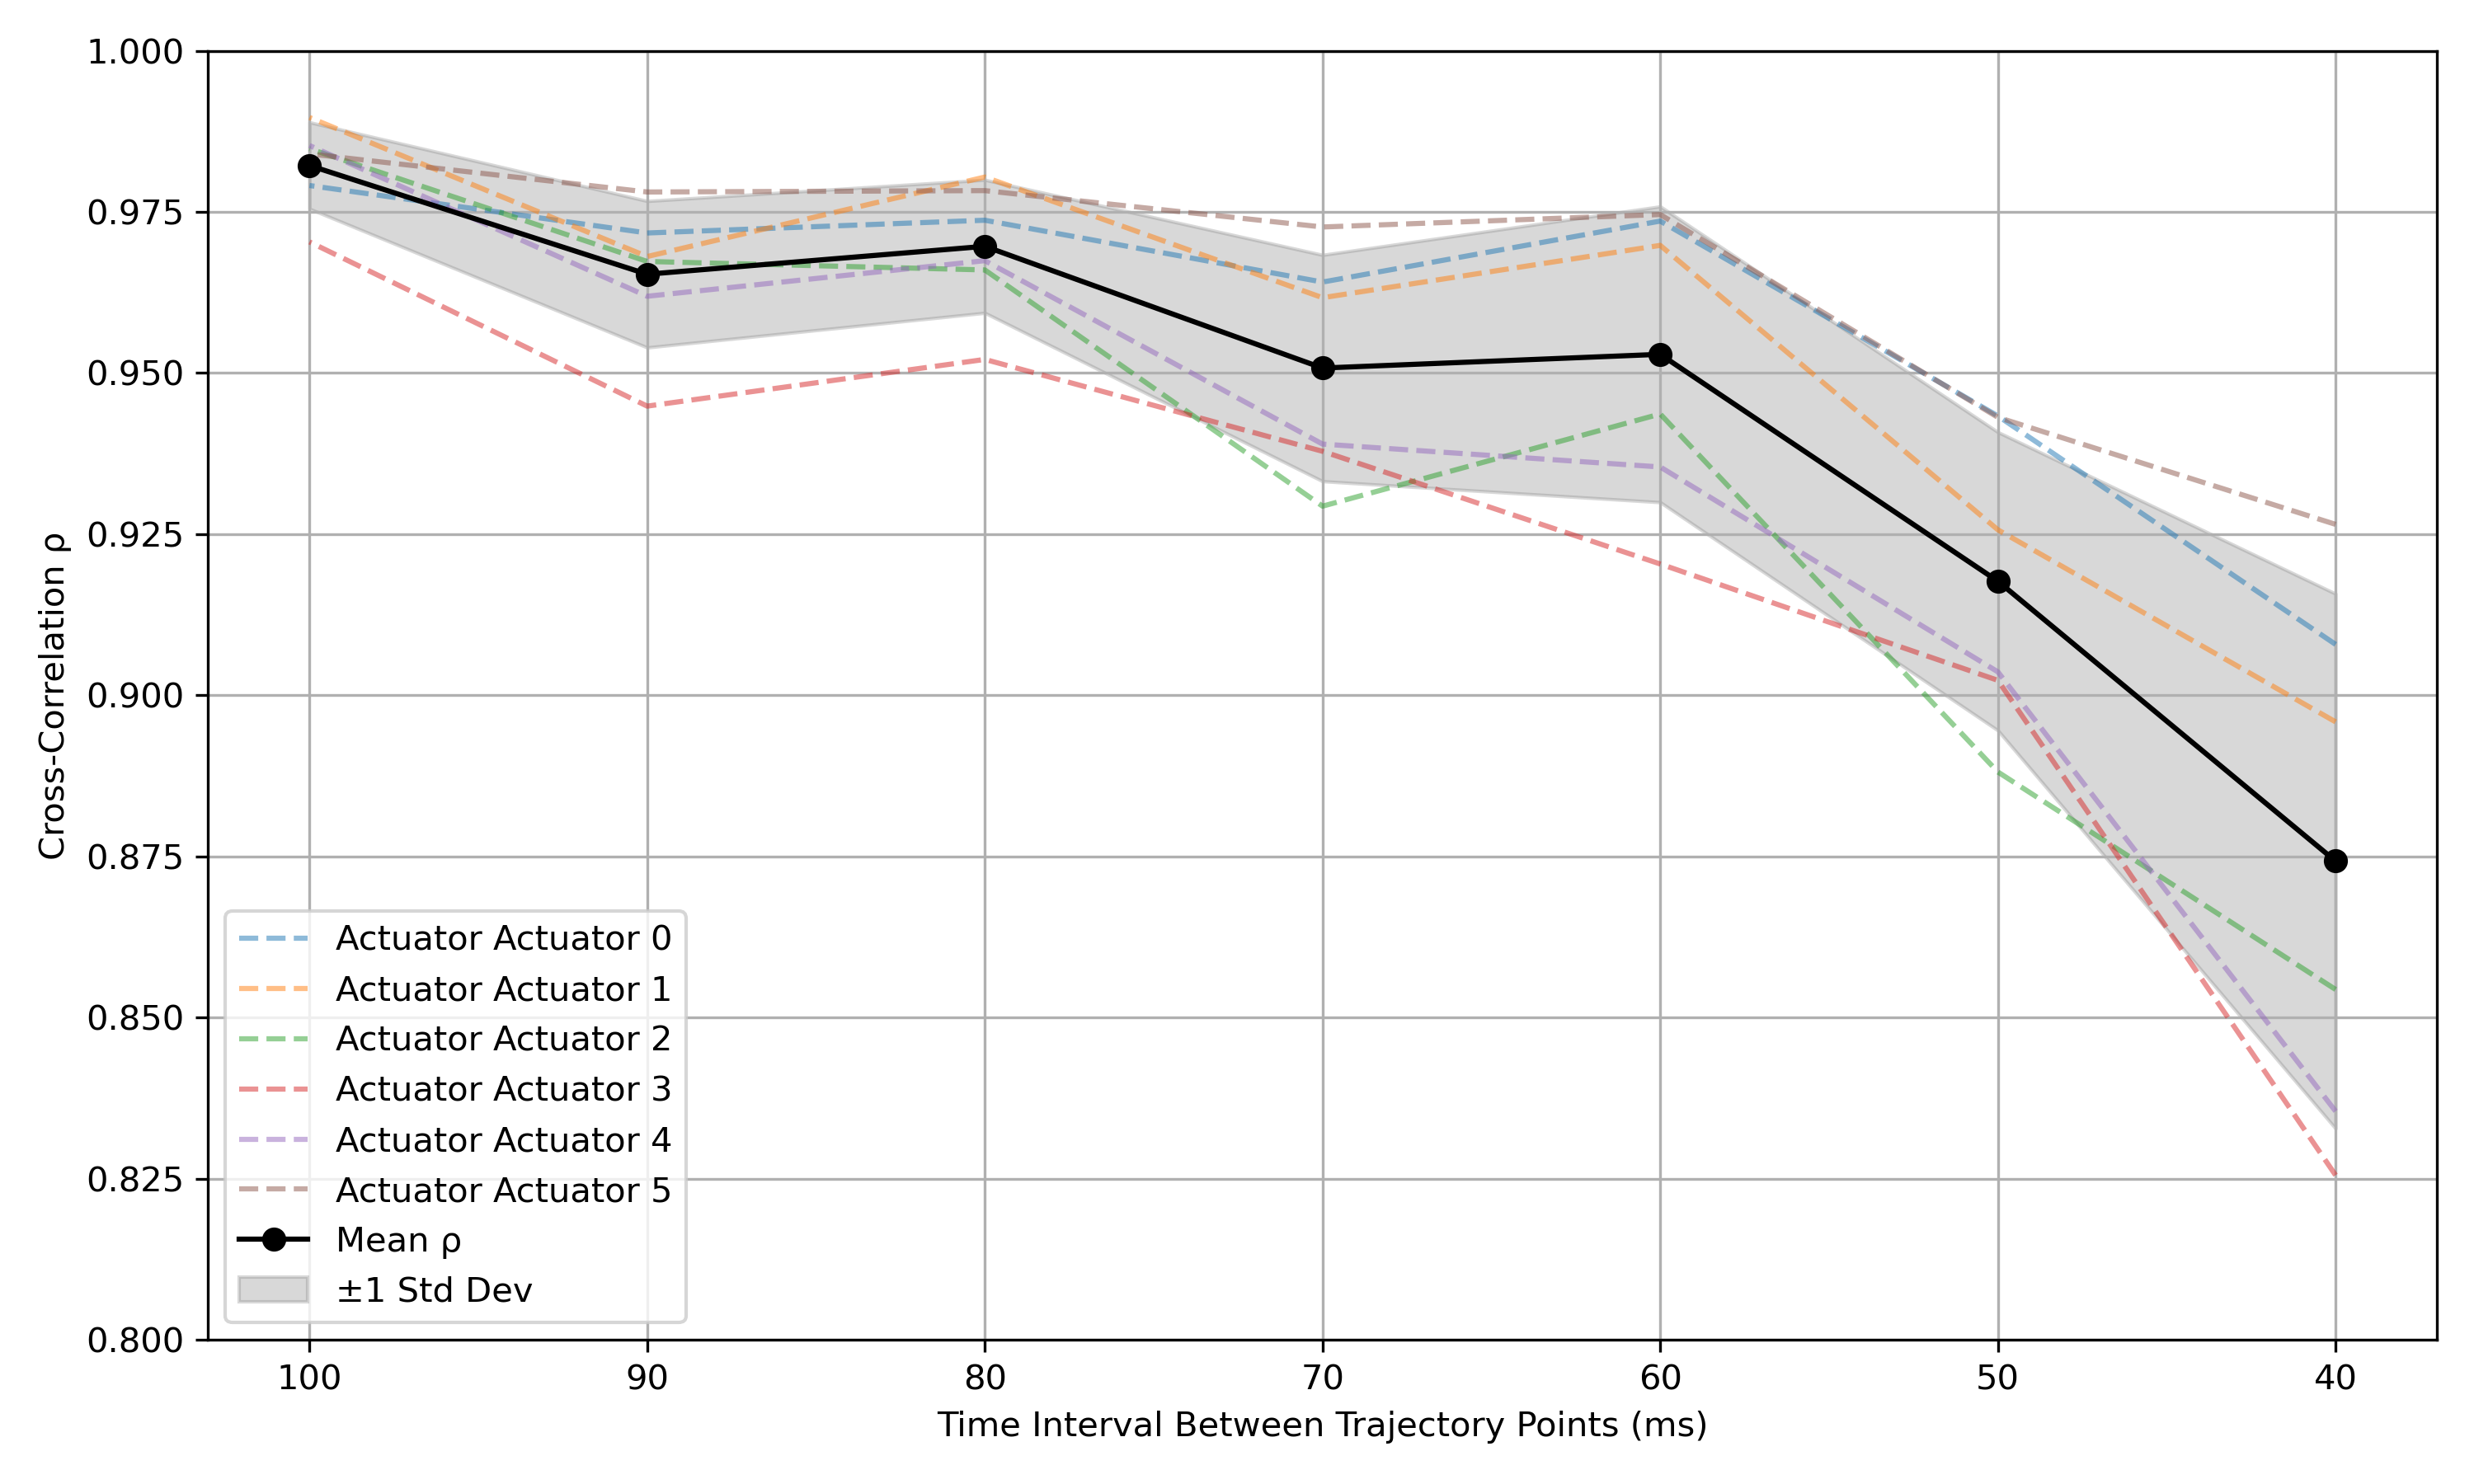
\includegraphics[width=0.6\textwidth]{figures/actuator_rhos.png}
    \caption{Cross-correlation coefficients across actuators for different time intervals.}
    \label{fig:actuator_rhos_2}
\end{figure}

\subsection{Force analysis}

\subsubsection{Maximum force}

The robot's vertical force generation capabilities were assessed using manual control mode normally used to set the robot's home position during calibration. 
The platform was driven at its highest height under active force feedback while avoiding structural failure. The upper bound of the robot's vertical force 
output was constrained by the stiffness of the upper jaw structure, which visibly bent under high vertical force. Table~\ref{tab:max_force} shows the 
maximum forces recorded by the three load cells during this test, see Figure~\ref{fig:load_cells_axis}.
for the load cell positions. The results shows that most of the vertical force is applied to the back load cells, which reflects the 
anatomical load pattern during full occlusion, where the molars bear the majority of chewing forces. Similarly for the antero-posterior force ($F_y$) where most of it 
is applied on the front load cell, i.e. the incisors. The total vertical, lateral and antero-posterior force output of the robot are well within the average 
forces during healthy human chewing \cite{shear_force}, although $F_z$ is below the maximum bite force from Table~\ref{tab:functional_criteria}.
\begin{table}[H]
    \centering
    \begin{tabular}{p{4cm} p{2cm} p{2cm} p{2cm}}
        \toprule
        \textbf{Load Cell} & \textbf{$F_{z,max}$ (N)} & \textbf{$F_{y,max}$ (N)} & \textbf{$F_{x,max}$ (N)} \\
        \midrule
        Back Right Load Cell & 124.63 & 59.64 & 123.85 \\
        Back Left Load Cell & 124.63 & 23.95 & 67.84  \\
        Front Load Cell & 66.28 & 81.38 & 123.07  \\
        \midrule
        \textbf{Total Force} & \textbf{315.98} & \textbf{103.08} & \textbf{125.71} \\
        \bottomrule       
    \end{tabular}
    \caption{Maximal forces recorded by the load cells during the force test.}
    \label{tab:max_force}
\end{table}

\subsubsection{Force feedback distribution}

To evaluate the spatial resolution of the force sensing system, we applied a simple vertical trajectory while placing a piece of gum-like material 
at three distinct positions between the teeth: back right, front, and back left. The vertical force output from each of the three load cells was 
recorded and shown in Figure~\ref{fig:force_distribution_gum}.

The plot clearly shows three distinct peaks corresponding to the three test positions, confirming the system's capability to localize force application 
across the dental arch. Additionally, when force is applied at the back, the front load cell registers a smaller secondary response. This is consistent 
with the mechanical coupling in the mounting structure, as the front load cell is physically situated between the two rear ones.

\begin{figure}[H]
    \centering 
    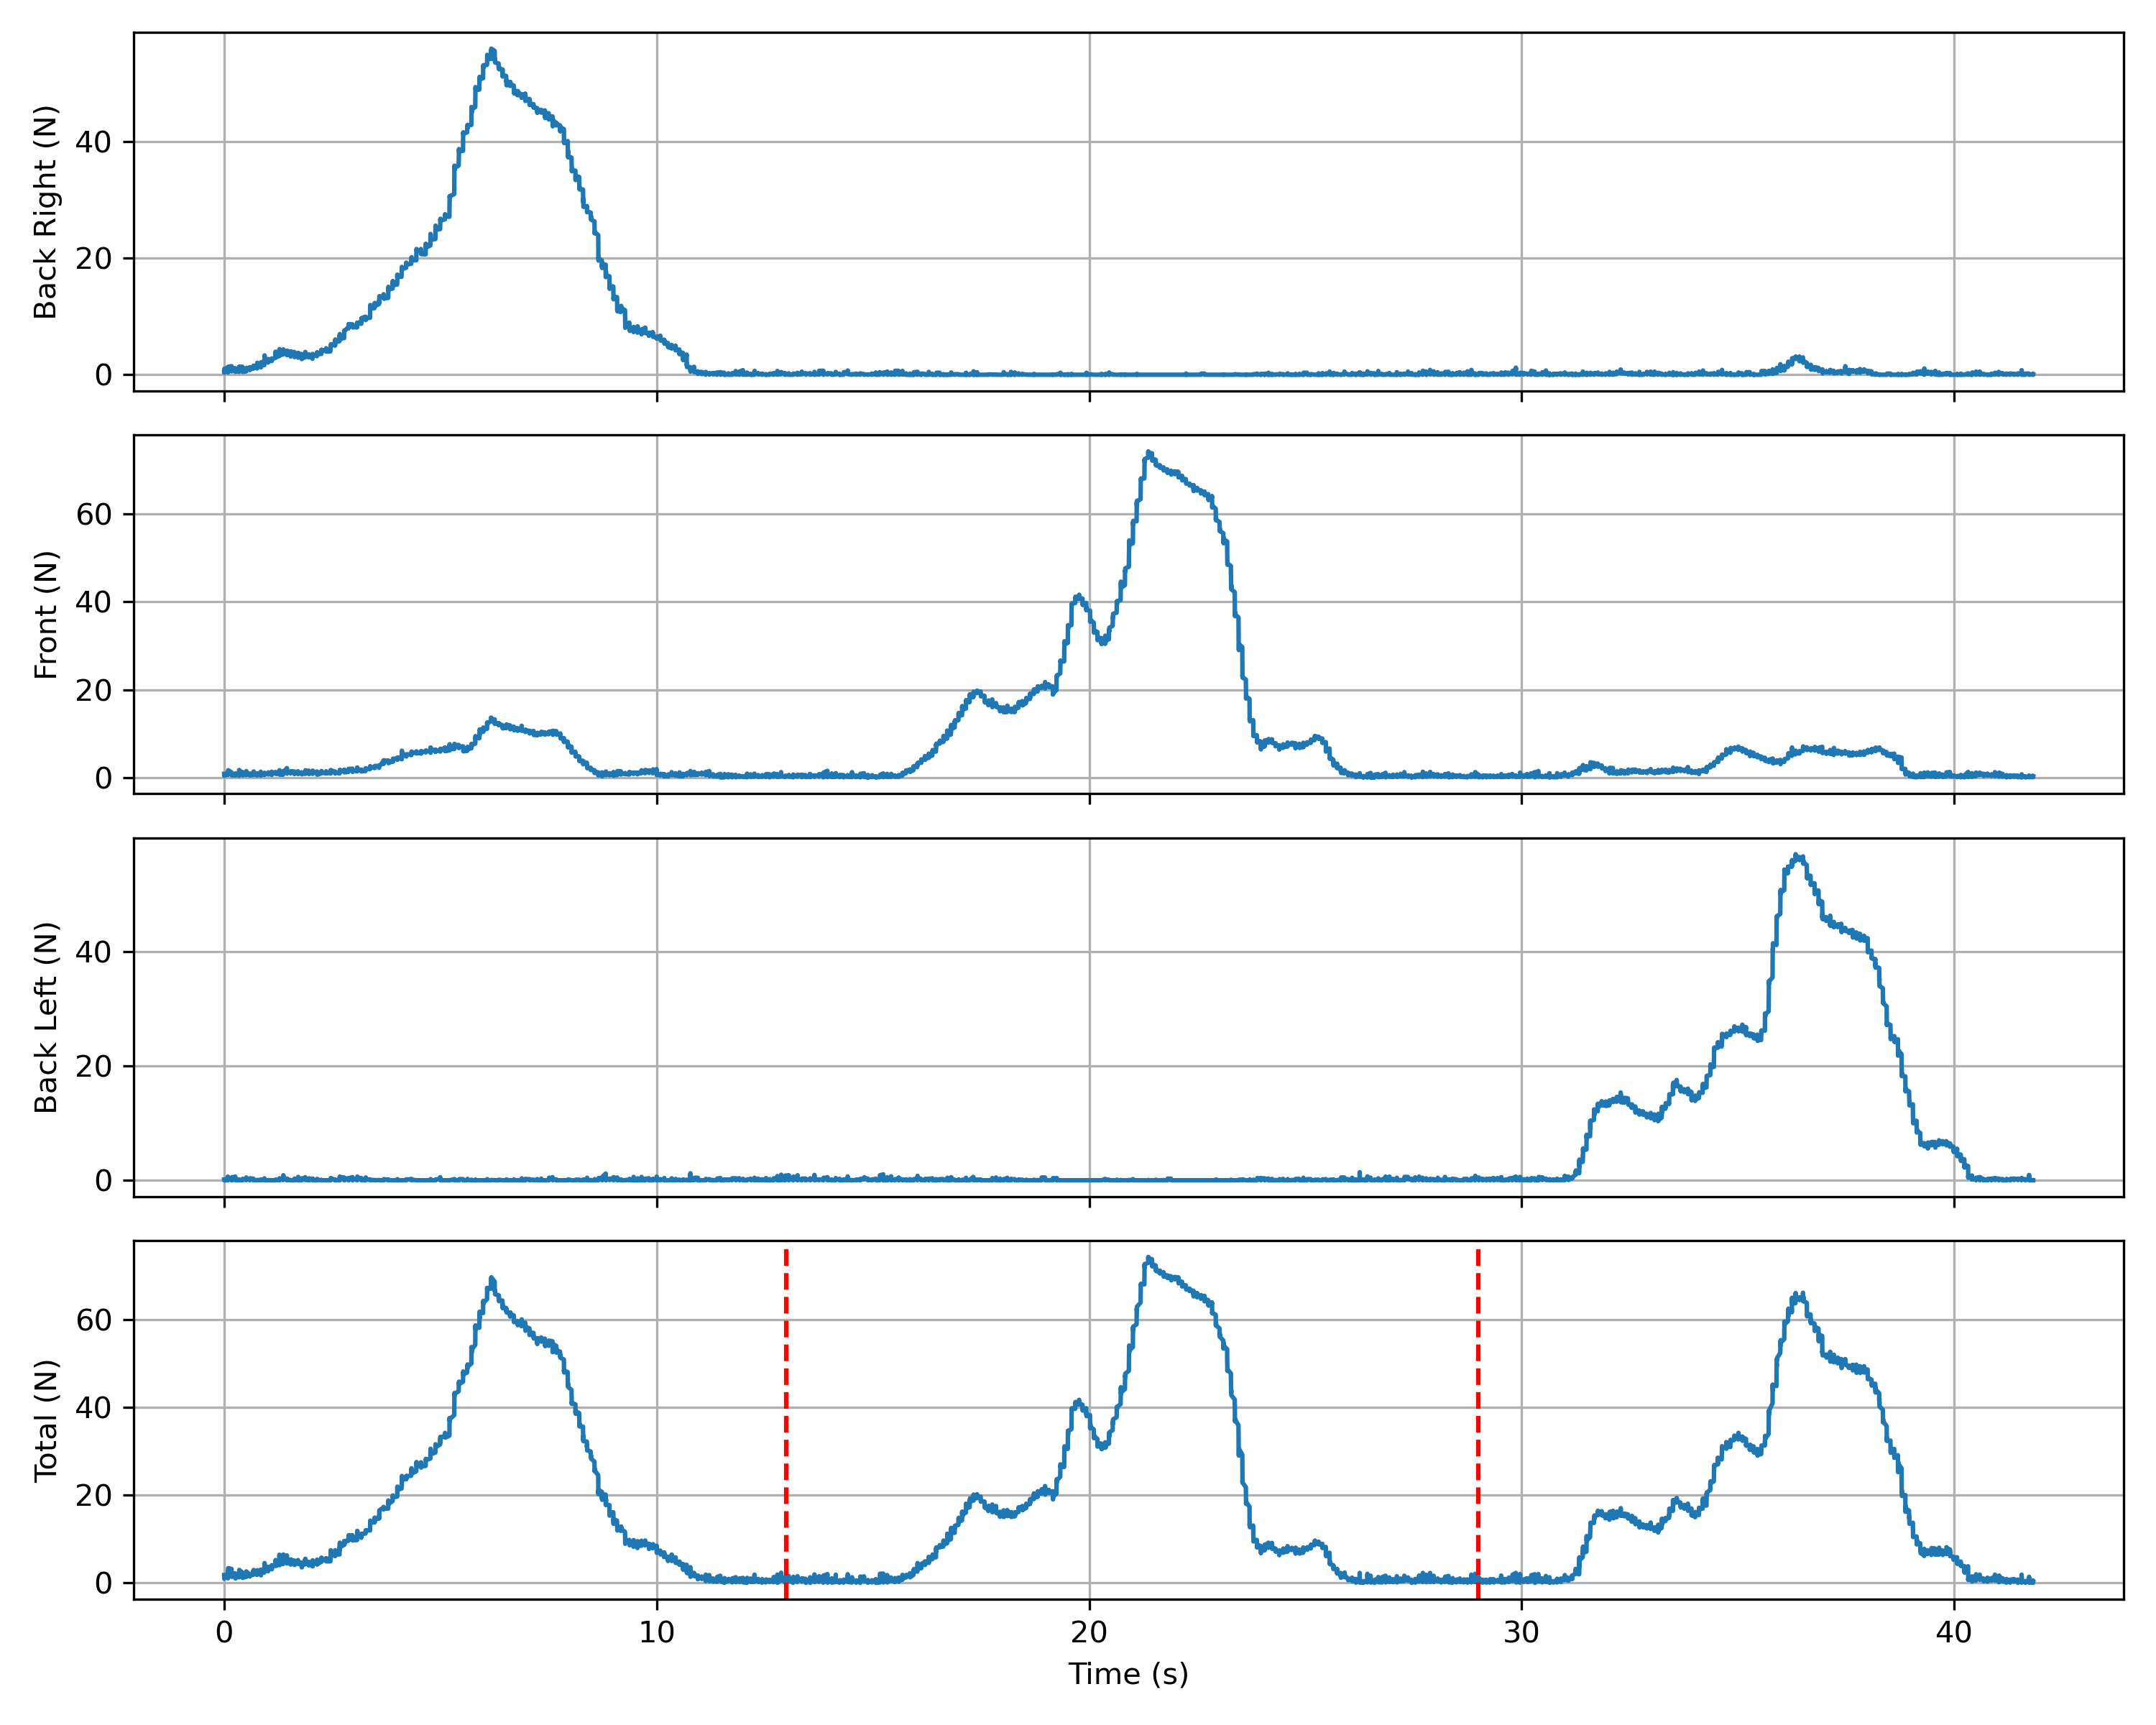
\includegraphics[width=0.7\textwidth]{figures/ForceDistributionGum.png}
    \caption{Vertical force output across three load cells during chewing with localized gum placement.  
    The red lines separate the three gum positions: back right, front, and back left.}
    \label{fig:force_distribution_gum}
\end{figure}

\subsection{Scalability and modularity}
A central goal of the project was to build a scalable platform for future modules such as a tongue, saliva pumps, and an esophagus. As described in 
Section~\ref{sec:mechanical_design}, the mechanical design already accommodates these additions, including space for internal cameras to observe the 
chewing process. A rendering of the proposed tongue module is shown in Figure~\ref{fig:tongue}. These design decisions were made in collaboration with 
project supervisor Benhui Dai.

\begin{figure}[H]
\centering
\begin{minipage}{.45\textwidth}
  \centering
  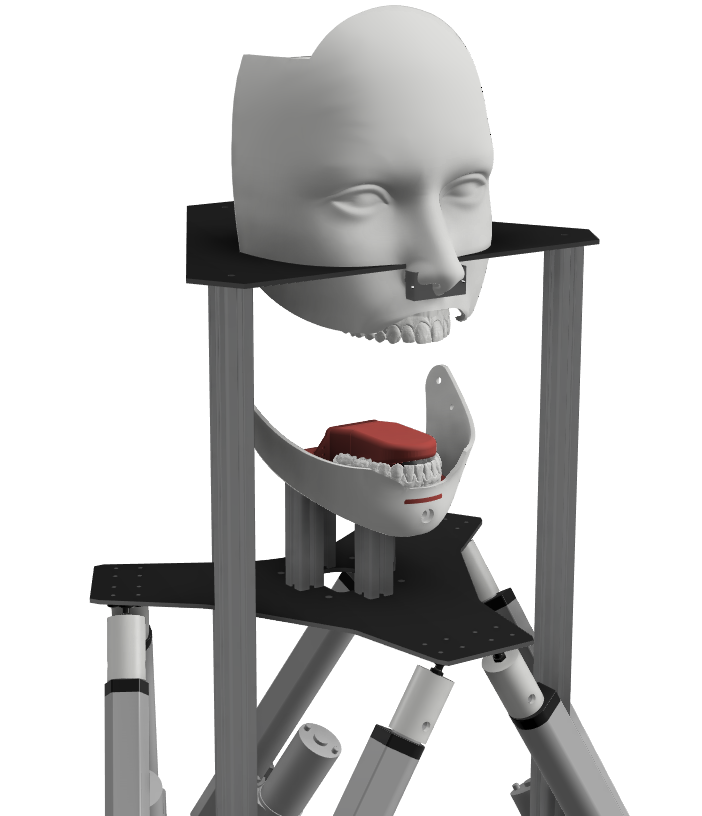
\includegraphics[height=5cm]{figures/tongue_front.png}
  \subcaption{}
  \label{fig:tongue_front}
\end{minipage}
\begin{minipage}{.45\textwidth}
  \centering
  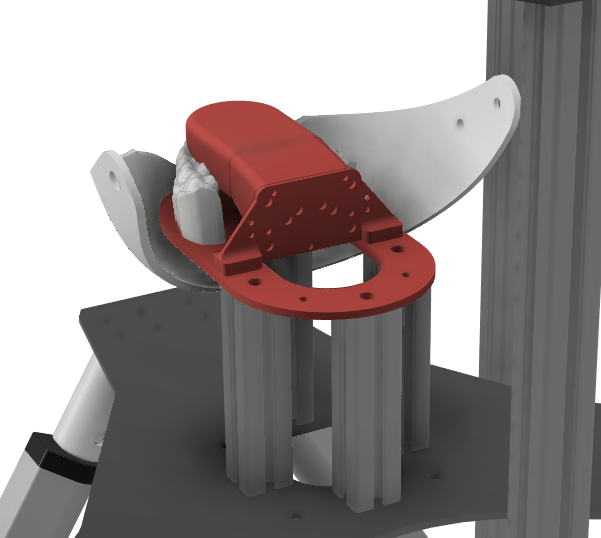
\includegraphics[height=5cm]{figures/tongue_back.png}
  \subcaption{}
  \label{fig:tongue_back}
\end{minipage}
\caption{Future tongue module rendering. (a) Front view, (b) Back view. }
\label{fig:tongue}
\end{figure}

The control system, detailed in Section~\ref{sec:control}, was developed with similar modularity in mind. Its finite-state machine architecture supports 
the easy integration of new components such as actuators and sensors for additional subsystems.

The robot's modularity also extends to the dental elements. Maxillary and mandibular teeth are mounted on replaceable acrylic adaptors, allowing for 
rapid testing of different dentitions. Combined with flexible trajectory loading, this makes the system suitable for a wide range of experimental and clinical scenarios.
